\documentclass{article}
\usepackage{amsmath}
\usepackage[utf8]{inputenc}
\usepackage{float}
\usepackage{epsfig,graphicx}
\usepackage{xcolor,import}
\usepackage[german]{babel}
\usepackage{textcomp}

\begin{document}


\thispagestyle{empty}
			\begin{center}
			\Large{Fakultät für Physik}\\
			\end{center}
\begin{verbatim}


\end{verbatim}
							%Eintrag des Wintersemesters
			\begin{center}
			\textbf{\LARGE WINTERSEMESTER 2014/15}
			\end{center}
\begin{verbatim}


\end{verbatim}
			\begin{center}
			\textbf{\LARGE{Physikalisches Praktikum 1}}
			\end{center}
\begin{verbatim}




\end{verbatim}

			\begin{center}
			\textbf{\LARGE{PROTOKOLL}}
			\end{center}
			
\begin{verbatim}





\end{verbatim}

			\begin{flushleft}
			\textbf{\Large{Experiment (Nr., Titel):}}\\
							%Experiment Nr. und Titel statt den Punkten eintragen
			\LARGE{1. Messen - Messfehler}	
			\end{flushleft}

\begin{verbatim}

\end{verbatim}	
							%Eintragen des Abgabedatums, oder des Erstelldatums des Protokolls
			\begin{flushleft}
			\textbf{\Large{Datum:}} \Large{17.10.2014}
			\end{flushleft}
			
\begin{verbatim}
\end{verbatim}
							%Namen der Protokollschreiber
		\begin{flushleft}
			\textbf{\Large{Namen:}} \Large{Veronika Bachleitner, Erik Grafendorfer}
			\end{flushleft}

\begin{verbatim}


\end{verbatim}
							%Kurstag und Gruppennummer, zb. Fr/5
			\begin{flushleft}
			\textbf{\Large{Kurstag/Gruppe:}} \Large{Fr/1}
			\end{flushleft}

\begin{verbatim}






\end{verbatim}
							%Name des Betreuers, das Praktikum betreute.
			\begin{flushleft}
			\LARGE{\textbf{Betreuer:}}	\Large{SETMAN}	
			\end{flushleft}
%		\begin{figure}[!h]
%\def\svgwidth{70mm}
%\import{section1/}{nonne.eps_tex}
%\end{figure}
%$\pm$
%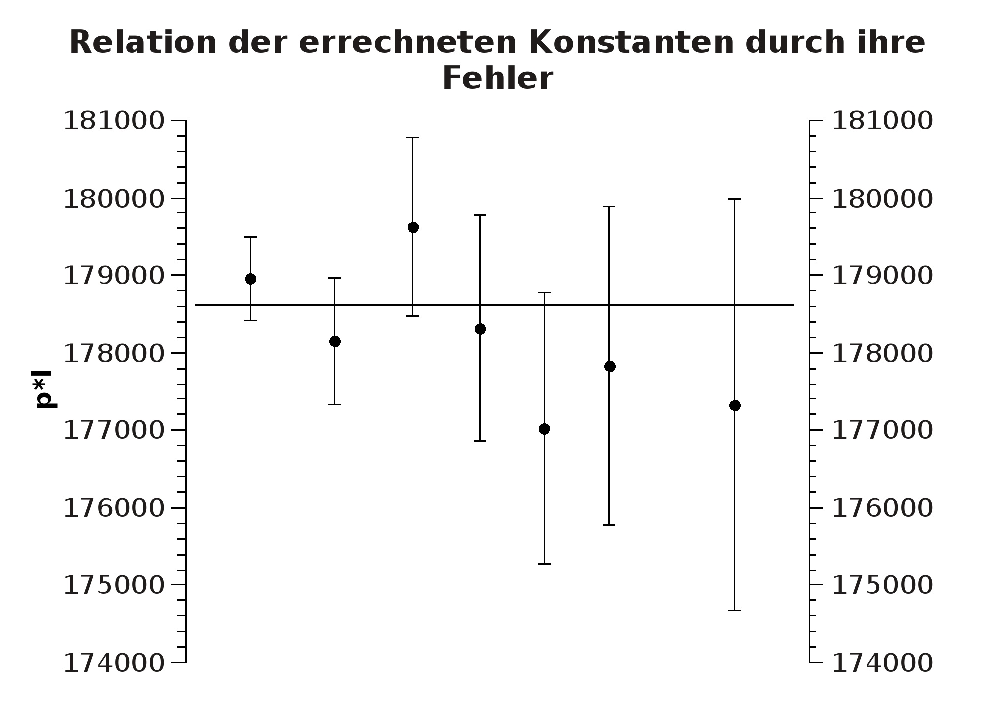
\includegraphics[scale=1,angle=-90]{Graph1.eps}[!h]
\section{Pendel}	
\subsection{Aufgabenstellung}
Es soll die Erdbeschleunigung aus Messungen der Periodendauer eines einfachen Fadenpendels bestimmt werden. Dazu werden 2 Messreihen durchgeführt: Einmal 10 Einzelmessungen als Messreihe; einmal eine Messung von 10 aufeinander folgenden Schwingungen.
\subsection{Grundlagen zum Experiment}
Das Fadenpendel stellt die experimentelle Näherung an ein mathematisches Pendel dar. Bei einem mathematischen Pendel ist die gesamte Masse im Schwerpunkt, die Aufhängung ist starr und reibungsfrei, sowie masselos.
\subsubsection*{Berechnung der Erdbeschleunigung}
Aus der Schwingungsdauer des Pendels können wir die lokale Erdbeschleunigung g näherungsweise berechnen. Wir verwenden für kleine Auslenkungswinkel $\alpha$ die Näherung Sin[$\alpha$] $\approx$ $\alpha$. 
Für die Schwingungsdauer T, die Frequenz f und die Pendellänge l gilt:

\begin{align}
T=\frac{1}{f}=2 \pi\sqrt{\frac{l}{g}} \\
g=4\pi^2\frac{l}{T^2}
\end{align}
\subsection{Material und Methoden / Versuchsaufbau}
Wir arbeiten in drei Gruppen mit drei verschiedenen Pendeln, die aus einer kleinen, schweren Kugel an einem langen Faden bestehen. Die Gruppen arbeiten mit verschieden langen Fäden, damit wir später unsere Ergebnisse für $T^2$ durch eine lineare Regression verbinden und eine genauere Näherung für den Faktor 
\begin{equation*}
\frac{4}{\pi^2 \cdot g} 
\end{equation*} erhalten. 
Wir verwenden eine Stoppuhr, die auf 0.01s genau messen kann.\\
Wir messen die Länge des Fadens von der Mitte der Stange, an der der Faden hängt, bis zur Mitte der Kugel, die wir als ihren Schwerpunkt idealisieren. Wir erhalten \\
 \begin{center}
 l=(0.928$\pm$0.001)m
 \end{center}
 mit der Unsicherheit $\Delta$l=0.001m als der kleinsten Einzeichnung auf dem Maßband.

\subsection{Durchführung des Experiments}
Wir messen zehn Mal immer neu ausgeführte Schwingungen des Pendels und ein Mal zehn aufeinanderfolgende Schwingungen mit einer Stoppuhr der Unsicherheit $\pm$0.01s. Dabei verwenden wir nur kleine Auslenkungen damit wir nachher in der Lösung der Schwingungsgleichung den Sinus mit dem kleinen Winkel nähern können. Die größte Unsicherheit stellen natürlich die Experimentatoren selbst dar, da sie ohne automatische Hilfsmittel, nur mit ihren Augen die Messungen starten und stoppen. Um diese Unsicherheit zu minimieren machen wir ein mal viele Messungen und messen einmal viele Schwingungen.
\subsection{Ergebnisse}
\begin{table} [H]
\caption{Messungen einzelner Schwingungen}
\begin{center}
\begin{tabular}{|c|c|}
\hline \\
Durchgang & Schwingungsdauer[($\pm$0.02s)]\\
\hline
 1&1.96\\
2&1.93\\
3&1.87\\
4&1.95\\
5&1.82\\
 6&1.93\\
7&1.92\\
 8&1.99\\
 9&1.9\\
 10&1.97\\
\hline $\Bar{T_{Einzel}}$ & 1.93 \\
\hline


\end{tabular} \\
\vspace{1cm}
Messung von 10 konsekutiven Schwingungen:\\
\vspace{1cm}
$T_{Serie}$=(19.36 $\pm$0.01)s
\end{center}
\end{table}


Wir berechnen die Unsicherheit der Erdbeschleunigung $\Delta g$ laut dem Gaußschen Fehlerfortpflanzungsgesetz. Wir berechnen diese 2 Mal, nachdem wir unterschiedliche Näherungswerte und Unsicherheiten für die Schwingungsdauer erhalten wenn wir sie 10 Mal einzeln oder 10 Mal in Folge messen.
Die Standardabweichung der Messserie von 10 Einzelschwingungen ist größer als die Auflösung der Stopuhr, also verwenden wir sie dort $\sigma$ = $\Delta$T=0.02s

\begin{align}
\Delta g=\sqrt{(\frac{\delta g}{\delta l})^2\Delta l^2 + (\frac{\delta g}{\delta T})^2\Delta T^2}
\end{align} \\
Für die 10 Einzelmessungen ist
\begin{equation}
T_{Einzel,genaehert} = (1.93 \pm 0.02)s
\end{equation}
Damit:
\begin{equation}
\Delta g_{Einzel,genaehert} = 0.067 \frac{m}{s^2}
\end{equation}
 Schließlich:
 \begin{equation}
 g{Einzel}=(9.84\pm0.07)\frac{m}{s^2}
 \end{equation}



\begin{equation}
T_{Serie,genaehert} = (1.94 \pm 0.01)s
\end{equation}
Damit:
\begin{gather}
\Delta g_{Serie,genaehert} = 0.0376 \frac{m}{s^2} \\
 g_{Serie} = (9.73\pm0.04)\frac{m}{s^2}
\end{gather}

Wir berechnen noch einen gewichteten Mittelwert aus den Einzelmessungen und der Messserie:
 \begin{gather}
 \frac{1}{\Delta T_{Einzel}}:\frac{1}{\Delta T_{Serie}}=g_1:g_2 \\
 \frac{1}{0.02}:\frac{1}{0.01}=50:100=1:2=g_1:g_2 \\
 T_g=\frac{T_{Einzel}g_1+T_{Serie}g_2}{g_1+g_2}=\frac{1.93+1.94\cdot2}{1+2} \\
 T_g=1.937s \\
 g_g=9.77 \\
 \Delta g_g= \sqrt{\frac{\Sigma^k_{j=1}( \bar{g_j} \bar{g_g} )^2 \cdot g_j}{(k1)\Sigma^k_{j=1}g_j} } \\
 \Delta g_g=0.053 \frac{m}{s^2}
 \end{gather}
 Unser Endergebnis:
 \begin{equation}
 g=g_g\pm \Delta g_g = (9.77 \pm 0.053)\frac{m}{s^2}
 \end{equation}

Schließlich verwenden wir die genauesten Paare von Pendellänge und Schwingungsdauer von allen drei Gruppen, plus einem Paar, das uns die Praktikumsleiterin zur Verfügung stellte, um eine lineare Regression über die Pendellängen durch die Quadrate der Schwingungsdauern zu fitten. Wir verwendeten QtiPlot 0.9.8.9 für die Berechnung und die Darstellung. \\

 Die Steigung der gefitteten Gerade ist 4.1558, daraus:
 \begin{equation}
 g=9.5 \frac{m}{s^2}
 \end{equation}
 Wir vermuten, dass die anderen Gruppen schlecht gemessen haben und der Wert darum so weit vom Literaturwert abweicht.
\begin{figure}


\centering
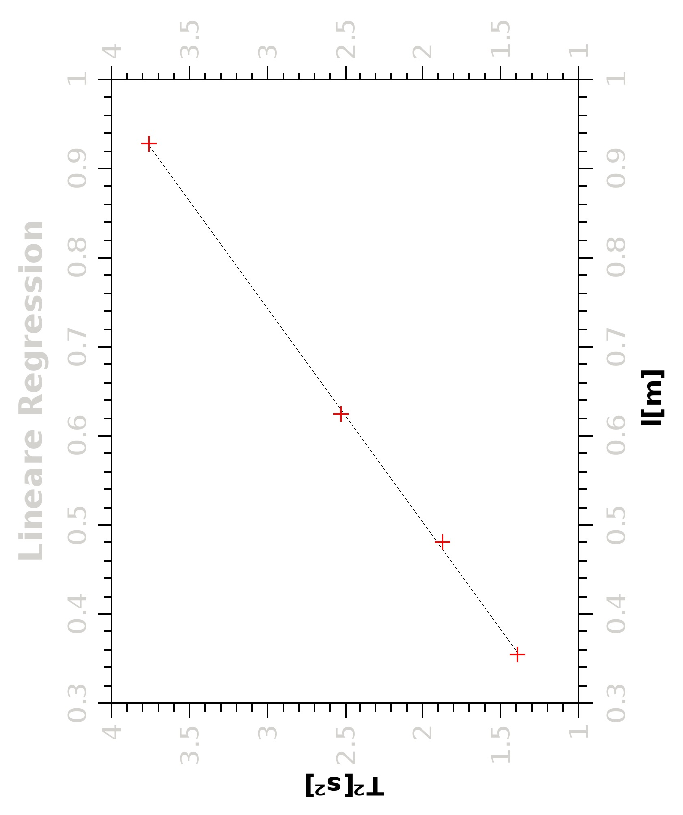
\includegraphics[scale=0.8,angle=-90]{LinearReg.eps} \\
\includegraphics[scale=0.5,angle=0]{regressiondata.eps}
\caption{Lineare Regression}

\end{figure}
\subsection{Diskussion}
Unsere ermittelten Ergebnisse für die Erdbeschleunigung liegen mit ihren Unsicherheiten erstens sehr schön beieinander, im 1$\sigma$Intervall der jeweils anderen, also können wir beiden Messungen vertrauen, und weiter liegen beide sehr nah am erwarteten Wert von 9.81$\frac{m}{s^2}$. Unbeachtet blieben systematischen Fehler, die wir unvermeidlich begangen haben, wie die Unsicherheit durch das menschliche Auge, die Näherung des Sinus durch den Winkel, die Eigenschwingungen des Pendelapparats und andere missachtete Fehler. Da sich die 1$\sigma$ Bereiche der unterschiedlichen Messungen aber überlappen, können wir nicht sagen, welche Methode ein signifkant besseres Ergebnis liefert.
\section{Mechanische Messungen}
\subsection{Aufgabenstellung}
Es soll der Durchmesser eines Kupferdrahtes mit verschiedenen Methoden gemessen werden. Verwendet werden eine Schublehre, eine Mikrometerschraube und ein Mikroskop mit Okularmaßstab.\\
Ferner sollen 3 Winkel eines Metall-Dreiecks mit einer Winkellehre gemessen werden.

\subsection{Grundlagen zum Experiment}
\subsubsection*{Schublehre}
Mit der Schublehre können Längen mit einer Genauigkeit von 0,05mm gemessen werden. Es gibt eine Hauptskala in Millimeter sowie einen Nonius auf einem beweglichen Schieber. Auf der verwendeten Schublehre sind 20 Teile der Noniusskala auf 39mm der Hauptskala aufgeteilt. Das bedeutet, dass 1mm durch 20 geteilt wird und wir somit die besagte Genauigkeit von $\pm$0,05mm erhalten.\\
%Das hast du so gut beschrieben, Vero, dass ich den Ruf nach einer Abbildung im Äther verhallen lasse.
\subsubsection*{Mikrometerschraube}
Mit der Mikrometerschraube können Längen mit einer Genauigkeit von $\pm$0,01mm gemessen werden.

\subsubsection*{Mikroskop}
Am Mikroskop verwenden wir das gelbe Objektiv mit der Vergrößerung von 10x0.25 und einen geeichten Maßstab von 2mm Länge mit Genauigkeit $\pm$0.01mm um die Dicke des Drahtes noch genauer messen zu können. 
\subsubsection*{Winkellehre}
Um mit der Winkellehre zu messen legt man das zu messende Objekt zwischen die beiden Mess-Schenkel und passt die Schenkel an die Größe an. Das Ergebnis ist wie bei der Schublehre an einer Hauptskala mit Nonius abzulesen.

\subsection{Material und Methoden / Versuchsaufbau}
Wir messen einen gespannten Kupferdraht mit den verschiedenen erwähnten Instrumenten. Zu diesem einfachen Aufbau gibt es wohl nicht mehr zu sagen. Wir messen auch ein metallenes Dreieck mit einem Goniometer.
\subsection{Durchführung des Experiments}
Bei unserer ersten Messung mit der Schublehre messen wir 0.45mm, was von den folgenden Messungen stark abweicht - wir haben wohl beim ersten Kontakt mit dem Instrument gepfuscht und verwerfen den Messwert! Die restlichen Messungen verlaufen problemlos.
\subsection{Ergebnisse}

\begin{table}
\centering
\begin{tabular}{|c|c|c|}
\hline
n&$l_1$[mm]&$l_2$[mm]\\
\hline
\hline
1&0.25&0.2\\
2&0.2&0.21\\
3&0.25&0.2\\
4&0.2&0.2\\
5&0.25&0.2\\
\hline 
$\bar{l}$&0.23&0.20\\
\hline
\end{tabular}
\caption{Messungen mit der Schublehre und der Mikrometerschraube}
\end{table}

Wir messen die Dicke des Kupferdrahtes an verschiedenen Stellen  fünf Mal mit der Schublehre, fünf Mal mit der Mikrometerschraube und ein Mal mit dem Mikroskop.  Die Messungenauigkeit der Schublehre liegt mit 0.05mm über dem Standardfehler von 0.012mm, darum ist die Länge hier

\begin{equation}
l_1=(0.23\pm0.05)mm
\end{equation}
\\
Bei der Mikrometerschraube ist die Messungenauigkeit mit 0.1mm ebenfalls größer als der Standardfehler der Messungen von 0.001mm, also ist hier \\ 
\begin{equation}
l_2=(0.2\pm0.1)mm. 
\end{equation}
Die Messung mit dem Mikroskop ergab eine Länge $l_3$ von
\begin{equation}
l_3=(0.19 \pm 0.01) mm
\end{equation}
Nachdem wir mit drei verschiedenen Instrumenten gemessen haben, wollen wir noch ein gewichtetes Mittel aus diesen drei Ergebnissen ermitteln um all unsere Messungen in das Endergebnis einfließen zu lassen. Dabei verwenden wir für die Gewichtungsfaktoren:
\begin{equation}
\frac{1}{\Delta l_1}:\frac{1}{\Delta l_2}:\frac{1}{\Delta l_3}=g_1:g_2:g_3=20:10:100=2:1:10
\end{equation}
Nun:
\begin{gather*}
\bar{l_g}=\frac{\bar{l_1}g_1+\bar{l_2}g_2+\bar{l_3}g_3}{g_1+g_2+g_3} \\
\bar{l_g}=\frac{0.23\cdot2+0.2\cdot1+0.19\cdot10}{2+1+10} \\
\bar{l_g}=0.197mm \\
\Delta l_g= \sqrt{\frac{\Sigma^k_{j=1}( \bar{l_j} -\bar{l_g} )^2 \cdot g_j}{(k-1)\Sigma^k_{j=1}g_j} } \\
\Delta l_g= \sqrt{\frac{(0.23-0.197)^2\cdot2+(0.20-0.197)^2\cdot1+(0.19-0.197)^2\cdot10}{(3-1)(2+1+10)}}\\ = 0.014mm \\
\end{gather*}\\
Unser Endergebnis ist demnach:\\
\begin{equation}
l_g=\bar{l_g}\pm\Delta l_g = (0.197\pm0.014)mm
\end{equation}\\

Wir messen die drei Winkel am Dreieck als 45°15, 30°40' und 103°35', mit einer Unsicherheit, gegeben durch die Noniusskala am Goniometer, von $\pm$5'. Addiert ergeben die Winkel 179°30', was als unser Endergebnis stehen bleibt.
\begin{equation}
Winkelsumme=179^{\circ}30'\pm15'
\end{equation}
\subsection{Diskussion}
Die Messergebnisse mit den immer genaueren Instrumenten der Mikrometerschraube, der Schublehre und des geeichten Maßstabs am Mikroskop liegen in schöner Übereinstimmung miteinander, die Mittelwerte der Messergebnisse liegen innerhalb der Konfidenzintervalle der Messungenauigkeiten aller Instrumente. Wir können also mit hoher Wahrscheinlichkeit davon ausgehen dass wir genau gemessen haben. \\
Die Winkelsumme des Dreiecks ist zwar nicht die von der Mathematik geforderte Summe von 180°, aber es handelt sich schließlich um ein physikalisches Objekt und fehlerbehaftete Menschen, die zum ersten Mal mit solchen Instrumenten gemessen haben.
\section{Elektrische Messungen}
\subsection{Aufgabenstellung}
Im Gleichstrom messen wir Ströme und Spannungen in verschiedenen Schaltungen, mal spannungsrichtig, mal stromrichtig, um mit Augenmerk auf die Fehlergrenzen unserer Messgeräte zu sehen, ob wir unsere Messungen wegen der Innenwiderstände der Messgeräte überhaupt korrigieren müssen oder nicht.\\
Weiters messen wir in Parallel- und Serienschaltungen Widerstände und vergleichen sie mit den berechneten Werten.\\
Im Wechselstrom bauen wir einen Spannungsteiler und berechnen Spannungen und Ströme auch in einer modifizierten Schaltung mit einem Kondensator.
\\
\subsection{Grundlagen zum Experiment}
Spannung U: [U]=V (Volt)\\
Stromstärke I: [I]=A (Ampère)\\
Widerstand R: [R]=$\Omega$ (Ohm)\\

\subsubsection*{Gleichstrom}
Das Ohm'sche Gesetz: U=RI\\
\\
Für die Messung werden ein Ampèremeter (Stromstärke) und ein Voltmeter (Spannung) benötigt, wobei das Ampèremeter in Serie und das Voltmeter parallel zum Widerstand geschaltet wird. Der Grund dafür ist, dass a) das Ampèremeter einen kleinen Innenwiderstand hat, und bei Parallelschaltung ein zu großer Strom durch das Gerät fließen und es zerstören könnte; b) das Voltmeter einen hohen Innenwiderstand hat und bei Serienschaltung daher kaum noch Strom fließen würde.\\
\\
Man kann eine stromrichtige und eine spannungsrichtige Schaltung bauen. \\
Stromrichtigen Schaltung: Durch das Ampéremeter fließt derselbe Strom wie durch den Widerstand und die Spannung wird aufgeteilt, sodass das Voltmeter die Summe von zwei (verschiedenen) Spannungen misst.\\
Spannungsrichtige Schaltung: Das Voltmeter misst dieselbe Spannung wie am Widerstand und der Strom wird aufgeteilt, sodass das Ampéremeter den Gesamtstrom misst, anstatt des Stroms am Widerstand.

\subsubsection*{Wechselstrom}
Eine Spannungsquelle für Wechselstrom gibt eine zeitlich wechselnde Spannung U(t) aus. Zusätzlich zum Ohm'schen Widerstand (die sich idealerweise wie im Gleichstrom verhalten sollten) treten auch kapazitive und induktive Widerstände auf, wobei wir in diesem Fall nur einen zusätzlichen kapazitiven Widerstand betrachten.\\
Kapazitive Widerstände sind im Gegensatz zu Ohm'schen Widerständen frequenzabhängig und verursachen eine Phasenverschiebung zwischen Strom und Spannung. \\
Die Berechnung erfolgt mithilfe von komplexen Größen. Die gemessenen reellen Wechselstromgrößen sind dann die Beträge dieser komplexen Größen.


\subsection{Material und Methoden / Versuchsaufbau}
Als Ampèremeter wurde das Gerät FLUKE 175 verwendet; als Voltmeter das Gerät FLUKE 179.\\
\\
Spannungsrichtige Schaltung:\\
\includegraphics[scale=0.8]{1spannungsrichtig.eps}\\
\\
Stromrichtige Schaltung:\\
\includegraphics[scale=0.8]{1stromrichtig.eps}\\
\\
Parallelschaltung:\\
\includegraphics[scale=0.8]{parallelschaltung.eps}\\
\\
Serienschaltung:\\
\includegraphics[scale=0.8]{serienschaltung.eps}\\
\\
Wechselstrom:\\
\includegraphics[scale=0.8]{wechselstrom.eps}\\

\subsection{Ergebnisse}
\textbf{Spannungsrichtige Messung:}\\
$U_V$=(23.97 $\pm$ (0.15\%+2))V = (23.97 $\pm$ 0.06)V\\
$I_V$=(8.88 $\pm$ (1\%+3))mA = (8.88 $\pm$ 0.11)mA\\

\textbf{Stromrichtige Messung:}\\
$U_A$ =(24.00 $\pm$ (0.15\%+2))V = (24.00 $\pm$ 0.06)V\\
$I_A$ =(8.88m $\pm$ (1\%+3))mA = (8.88 $\pm$ 0.11)mA\\

\textbf{Die daraus errechneten Widerstände:}
$R_V$=$\frac{U_V}{I_V}$ = $\frac{24}{8.88*10^{-3}}$ =2.70k$\Omega$\\
$R_A$=$\frac{U_A}{I_A}$ = $\frac{24}{8.88*10^{-3}}$ =2.70k$\Omega$\\
\\
\textbf{Relativer Fehler:}\\
$\frac{\Delta U}{U}$=0.0025=0.25\%\\
$\frac{\Delta I}{I}$=0.0124=1.24\%\\
\\
\textbf{Relativer Fehler von R:}\\
\begin{gather}
\sqrt{(\frac{\Delta U}{U})^2+(\frac{\Delta I}{I})^2 }=\sqrt{0.0025^2+0.0124^2}=0.01264=1.27\%
\end{gather}
\\
\textbf{Widerstand R=(2.7 $\pm$ 0.04)k$\Omega$}\\
\\
Da unsere Resultate für den Widerstand in spannungsrichtiger und stromrichtiger Schaltung kaum einen Unterschied aufweisen, sind sie innerhalb der Fehlergrenze gleich.\\
\\
\textbf{Innenwiderstandskorrektur:}\\
In spannungsrichtiger Schaltung wurde U=23.97V und I=8.88mA gemessen.\\
In der Betriebsanleitung des FLUKE 179 (Voltmeter) wird ein Innenwiderstand von $R_i$$ \le $10M
$\Omega$ angegeben. Schon diese Zahl lässt darauf schließen, dass eine Innenwiderstandskorrektur nicht notwendig sein wird, wir wollen sie allerdings dennoch durchführen: \\
\\
Der Strom, der durch das Voltmeter fließt, ist: $\frac{23.97}{10^6}$=23.97$\mu$A\\
Der korrigierte Wert für den Strom: $I_{korr}$=(8.88-0.023)mA=8.86mA\\
Der korrigierte Wert für den Widerstand: $R_{korr}$=2.705k$\Omega$\\
\\
Dieser ist (schon ohne Unsicherheit) nur an der 3. Nachkommastelle verschieden vom vorherigen Wert, daher kann die Innenwiderstandskorrektur tatsächlich vernachlässigt werden.\\
\\
\subsubsection*{Parallelschaltung}
$U_P$=(23.92 $\pm$ (0.15\%+2))V=(23.92 $\pm$ 0.06)V\\
$I_P$=(17.83 $\pm$ (1\%+3))mA=(17.83 $\pm$ 0.21)mA\\
\\
$R_{P-Gesamt}$=$\frac{U_P}{I_P}$=$\frac{23.92}{17.83*10^{-3}}$=1.34k$\Omega$\\
\\
\textbf{Relativer Fehler:}\\
$\frac{\Delta U_P}{U_P}$=0.0025=0.25\%\\
$\frac{\Delta I_P}{I_P}$=0.0118=1.18\%\\
\\
\textbf{Relativer Fehler von $R_{P-Gesamt}$:}\\
\begin{gather}
\sqrt{(\frac{\Delta U_P}{U_P})^2+(\frac{\Delta I_P}{I_P})^2 }=\\
\sqrt{0.0025^2+0.0118^2}=0.01206=1.21%\\
\end{gather} \\
\textbf{Widerstand $R_P$=(1.34 $\pm$ 0.02)k$\Omega$}\\

\subsubsection*{Serienschaltung}

$U_S$=(23.99 $\pm$ (0.15\%+2))V=(23.92 $\pm$ 0.06)V\\
$I_S$=(4.45 $\pm$ (1\%+3))mA=(4.45 $\pm$ 0.08)mA\\
\\
$R_{S-Gesamt}$=$\frac{U_S}{I_S}$=$\frac{23.99}{4.45*10^{-3}}$=5.49k$\Omega$\\
\\
\textbf{Relativer Fehler:}\\
$\frac{\Delta U_S}{U_S}$=0.0025=0.25\%\\
$\frac{\Delta I_S}{I_S}$=0.0180=1.80\%\\
\\
\textbf{Relativer Fehler von $R_{S-Gesamt}$:}\\
\begin{gather}
\sqrt{(\frac{\Delta U_S}{U_S})^2+(\frac{\Delta I_S}{I_S})^2 }=\\
\sqrt{0.0025^2+0.0180^2}=0.01817=1.82\%
\end{gather}
\textbf{Widerstand $R_S$=(5.49 $\pm$ 0.10)k$\Omega$}\\
\\
\textbf{Innenwiderstandskorrektur:}\\
Der Strom, der durch das Voltmeter fließt, ist: $\frac{23.99}{10^6}$=23.99$\mu$A\\
korrigierter Wert für den Strom: $I_{korr}$=(4.45-0.024)mA=4.43mA\\
korrigierter Wert für den Widerstand: $R_{korr}$=5.41k$\Omega$\\
\\
Durch die Unsicherheit von 0.10k$\Omega$ ist auch hier die Innenwiderstandskorrektur vernachlässigbar.\\

\subsubsection*{Teilspannungen}
$U_{Rbekannt}$=(11.94 $\pm$ (0.15\%+2))V=(11.94 $\pm$ 0.04)V\\
$U_{Rx}$=(12.05 $\pm$ (0.15\%+2))V=(12.05 $\pm$ 0.04)V\\
\\
$R_{bekannt}$=2.7k$\Omega$\\
\\
Der Strom ist in beiden Fällen gleich. \\
I=$\frac{U_{Rbekannt}}{R_{bekannt}}$ = $\frac{U_Rx}{R_x}$\\
$R_x$ = $R_{bekannt}$$\frac{U_{Rx}}{U_{Rbekannt}}$ = 2.7 $\frac{12.05}{11.94}$ = 2.72k$\Omega$\\
\\
\textbf{Relativer Fehler der Teilspannungen:}\\
$U_{Rbekannt-Rel}$ = 0.0034=0.34\%\\
$U_{Rx-Rel}$ = 0.0034=0.34\%\\
\\
\textbf{Relativer Fehler von $R_x$:}\\
\begin{gather}	
\sqrt{(U_{Rbekannt-Rel})^2+(U_{Rx-Rel})^2)}=\sqrt{(2)*0.0034}=0.0048=0.48\%
\end{gather}
\textbf{Widerstand $R_x$=(2.72 $\pm$ 0.02)k$\Omega$}

\subsection*{Wechselstrom}
$I_{Gesamt}$=(5.07 $\pm$ (1.5\% + 3))mA = (5.07 $\pm$ 0.11)mA\\
$U_{Gesamt}$=(27.06 $\pm$ (1\%+3))V = (27.06 $\pm$ 0.30)V\\
$U_{Rx}$=(13.63 $\pm$ (1\%+3))V = (13.63 $\pm$ 0.17)V\\
$U_{Rbekannt}$=(13.49 $\pm$ (1\%+3))V = (13.49 $\pm$ 0.17)V\\
$R_{bekannt}$=2.7k$\Omega$\\
\\
\textbf{Aus den Teilspannungen:}\\
$R_x$=$R_{bekannt}$ * $\frac{U_{Rx}}{U_{Rbekannt}}$ = 2.7 * $\frac{13.63}{13.49}$ = 2.73k$\Omega$\\
$R_{Gesamt}$=$R_{bekannt}$ + $R_x$ = 5.43k$\Omega$\\
\\
\textbf{Aus Spannung und Strom:}\\
$R_{Gesamt-berechnet}$=$\frac{U_{Gesamt}}{I_{Gesamt}}$=$\frac{27.06}{5.07*10{^-3}}$=5.34k$\Omega$\\
\\

$I_{Gesamt}$=(3.57 $\pm$ (1.5\% + 3))mA = (3.57 $\pm$ 0.09)mA\\
$U_{Gesamt}$=(27.07 $\pm$ (1\%+3))V = (27.07 $\pm$ 0.30)V\\
$U_{Rbekannt}$=(9.57 $\pm$ (1\%+3))V = (9.57 $\pm$ 0.13)V\\
$U_C$=(25.43 $\pm$ (1\%+3))V = (25.43 $\pm$0.29)V\\
$R_{bekannt}$=2.7k$\Omega$\\
\\
Wir betrachten folgende Formeln:\\
$Z_{Gesamt}$ = $Z_R$ + $Z_C$ = R - $\frac{i}{\omega C}$ = R - i$X_C$\\
$U_C$=I*$X_C$\\
\\
\textbf{Aus den Teilspannungen:}\\
$X_C$=$R_{bekannt}$ $\frac{U_C}{U_{Rbekannt}}$ = 2.7 $\frac{25.43}{9.57}$ = 7.17k$\Omega$\\
\\
\textbf{Relativer Fehler:}\\
$U_{Rbekannt-Rel}$=0.0136=1.36\%\\
$U_{C-Rel}$=0.0114=1.14\%\\
\\
\textbf{Relativer Fehler von $X_C$:}\\
\begin{gather}
\sqrt{(U_{Rbekannt-Rel})^2+(U_{C-Rel})^2}=\\
\sqrt{(0.0136^2+0.0114^2)}=0.0177=1.77\% \\
X_C=(7.17 \pm 0.13)k\Omega
\end{gather} 
Aus den Teilspannungen ermittelter Wert für die Gesamtimpedanz:\\
$\lvert$ $Z_{Gesamt}$ $\rvert$ = sqrt($R^2$ + $X_C^2$) = sqrt($2.68^2$ + $7.12^2$) = 7.61k$\Omega$\\
\\
Aus Gesamtspannung und Gesamtstrom berechneter Wert für die Gesamtimpedanz:\\
$Z_{berechnet}$ = $\frac{U_{Gesamt}}{I_{Gesamt}}$ = $\frac{27.07}{3.57}$ = 7.58k$\Omega$\\

\textbf{Relativer Fehler der Teilspannungen:}\\
$U_{Gesamt-Rel}$ = 0.0111=1.11\%\\
$I_{Gesamt-Rel}$ = 0.0217=2.17\%\\
\\
\textbf{Relativer Fehler von $R_x$:}\\
\begin{gather}	
\sqrt{(U_{Gesamt-Rel})^2+(I_{Gesamt-Rel})^2)}=\sqrt{0.0111^2+0.0217^2}=0.0244=2.44\%
\end{gather}
\textbf{Impedanz $Z_{berechnet}$=(7.58 $\pm$ 0.19)k$\Omega$}\\
\\
Die Netzspannung beträt 230V, das bedeutet für die Frequenz f=50Hz. Daraus $\Omega$=2$\pi$f=314.16$s^{-1}$\\
\\
Aus X C=1/$\Omega$*C\\
\textbf{C=$\frac{1}{\Omega X_C}$ = $\frac{1}{314.16*7.12*10^3}$ = 22.66 F}

\subsubsection*{Grafische Darstellung}
\includegraphics[scale=0.8]{gaussebene.eps}

\subsection{Diskussion}
Unsere Messergebnisse stimmen sehr gut mit den berechneten Werten überein.\\
Die Innenwiderstandskorrekturen waren nicht notwendig.\\
Die Grafik der Gaußschen Zahlenebene zeigt, dass auch die Messergebnisse für die Spannungen beim Wechselstrom richtig waren.\\

\end{document}
